\chapter{Resultados}
\label{cap:resultados}

Este capítulo presenta lo que se midió en cada etapa de la cadena descrita en
el Capítulo~\ref{cap:diseno}, en el mismo orden en que la recorre la señal.
Primero se comparan los tres detectores sobre la traza continua y se mide la
calidad de sus recortes (objetivos OE1 y OE2: evaluar los detectores y
delimitar los eventos). Luego se mide la detección en las ventanas de test, se
presentan la búsqueda de la configuración y la validación cruzada del
clasificador (OE3: ajustar la red por transferencia de aprendizaje) y, por
último, el sistema completo aplicado a la traza continua (OE4: evaluar el
sistema integrado). El capítulo termina con las comprobaciones que se hicieron
para entender por qué el clasificador acierta menos en la traza que en test.
Todas las cifras se midieron sobre datos reales; su interpretación se discute
en el Capítulo~\ref{cap:discusion}.

% =====================================================================
\section{Comparación de detectores}
\label{sec:res-detectores}

Los tres detectores se evaluaron sobre la traza continua de FRE con los 125
eventos volcánicos del catálogo que tienen registro de las tres componentes:
36 VT, 52 LP y 37 TR. Los 6 AV y 48 IC que también tienen registro se informan
aparte. Todos se cuentan con la intersección descrita en la
Sección~\ref{subsec:protocolo-deteccion}: un evento está detectado si algún
intervalo del detector comparte al menos un instante con él, y una falsa
alarma es un intervalo que no toca ningún evento del catálogo. Las falsas
alarmas se cuentan por hora de registro (FP/h).

\subsection{Parámetros probados}
\label{subsec:res-parametros}

El Cuadro~\ref{tab:res-parametros} reúne los parámetros de cada detector, su
valor por defecto y los valores que se probaron. Solo se movieron parámetros
que expone la librería de cada detector, con el nombre que esta les da y
partiendo de su valor por defecto. Cada umbral se probó con 21 valores: 0,02,
0,03, 0,05 y de 0,10 a 0,95 cada 0,05. Los pasos son más finos bajo 0,10
porque ahí están los valores con que las redes detectan más.

{\small
\setlength{\tabcolsep}{4pt}
\begin{longtable}{>{\raggedright\arraybackslash}p{2.9cm}>{\raggedright\arraybackslash}p{4.5cm}>{\raggedright\arraybackslash}p{1.8cm}>{\raggedright\arraybackslash}p{3.0cm}}
\caption{Parámetros de cada detector. ``Por defecto'' es el valor que trae la
librería; en SeisBench, el que carga con los pesos ``original''.}\label{tab:res-parametros}\\
\cabecera{\textbf{Parámetro} & \textbf{Qué hace} & \textbf{Por defecto} & \textbf{Valores probados}}{4}
\multicolumn{4}{l}{\textit{PhaseNet (SeisBench)}}\\*
\texttt{P\_threshold} & Probabilidad mínima para aceptar una onda P & 0,3 & 0,02 a 0,95 \\
\texttt{S\_threshold} & Lo mismo para la onda S & 0,3 & 0,02 a 0,95, por separado del de P \\
\texttt{overlap} & Muestras que comparten dos ventanas seguidas de la red & 1500 (15\,s) & 500 a 2500 \\
\texttt{blinding} & Muestras que se descartan en cada borde de la ventana, donde la red ve señal hacia un solo lado & 250 por lado & 0 a 500 \\
\texttt{stacking} & Cómo se juntan las predicciones de ventanas que se solapan: promedio (\texttt{avg}) o máximo (\texttt{max}) & \texttt{avg} & \texttt{avg} y \texttt{max} \\
\midrule
\multicolumn{4}{l}{\textit{EQTransformer (SeisBench)}}\\*
\texttt{detection\_\allowbreak threshold} & Probabilidad mínima de la curva de detección & 0,3 & 0,02 a 0,95 \\
\texttt{P\_threshold}, \texttt{S\_threshold} & Probabilidad mínima de la onda P y de la onda S & 0,1 & 0,02 a 0,95, cada uno por separado \\
\texttt{overlap} & Igual que en PhaseNet & 3000 (30\,s) & 1000 a 5000 \\
\texttt{blinding} & Igual que en PhaseNet & 500 por lado & 0 a 1000 \\
\texttt{stacking} & Igual que en PhaseNet & \texttt{max} & \texttt{avg} y \texttt{max} \\
Filtro interno & Deja pasar 1--45\,Hz antes de entrar a la red & 1--45\,Hz & No se puede cambiar; viene con los pesos \\
\midrule
\multicolumn{4}{l}{\textit{STA/LTA (ObsPy)}}\\*
\texttt{nsta}, \texttt{nlta} & Largo de la ventana corta y de la larga & No tiene & 2 y 60\,s, sin cambio \\
\texttt{thres1}, \texttt{thres2} & Razón STA/LTA que enciende y que apaga el aviso & No tiene & 4,0 y 1,05, sin cambio \\
\texttt{freqmin}, \texttt{freqmax} & Banda del filtro previo & No tiene & 1 y 20\,Hz, sin cambio \\
\end{longtable}
}

Las redes no leen la traza de una vez, sino por ventanas: de 30\,s en PhaseNet
y de 60\,s en EQTransformer. Los parámetros \texttt{overlap},
\texttt{blinding} y \texttt{stacking} deciden cómo se recorren y se juntan esas
ventanas. A diferencia de los umbrales, cambian las curvas de probabilidad, así
que con cada combinación se volvió a correr la red sobre toda la traza. Se
omitieron las combinaciones con \texttt{overlap} menor que el doble de
\texttt{blinding}, porque descartan más de lo que se solapan y dejan tramos sin
predicción. Quedan 38 combinaciones por red; junto con los umbrales suman
16.758 casos en PhaseNet y 17.556 en EQTransformer. STA/LTA mantiene la
configuración que se eligió con un barrido en una evaluación anterior de este
trabajo, y usa solo la componente vertical.

Las dos redes reciben Z, N y E filtradas en 1--15\,Hz, la banda de la traza
publicada. También se probó la banda de 1--45\,Hz, la del filtro interno de
EQTransformer. Con ella PhaseNet necesita 73,9 falsas alarmas por hora para
llegar a 0,95, en vez de 69,0; EQTransformer llega al mismo máximo con su curva
de detección (0,864) y a uno menor con P y S (0,728 en vez de 0,736), y STA/LTA
detecta 105 volcánicos en vez de 106. Como no mejora a ningún detector, todo lo
que sigue usa 1--15\,Hz.

\subsection{Resultado con un umbral común}

Como punto de partida, el Cuadro~\ref{tab:res-umbral010} muestra los
detectores con el mismo umbral, 0,10, y las ventanas por defecto de las redes.
EQTransformer aparece dos veces porque entrega dos salidas: su curva de
detección y sus curvas de P y S. Las dos últimas columnas dan los volcánicos
que se contaban con el criterio anterior, con un aviso a 5 o a 10\,s del
inicio del evento.

{\small
\setlength{\tabcolsep}{3pt}
\begin{longtable}{>{\raggedright\arraybackslash}p{3.4cm}rrrrrrr}
\caption{Detección con umbral 0,10 en las redes. Volcánicos: detectados de 125.
Las dos últimas columnas usan el criterio anterior.}\label{tab:res-umbral010}\\
\cabecera{ & \multicolumn{5}{c}{\textbf{Intersección}} & \multicolumn{2}{c}{\textbf{Aviso a}} \\ \textbf{Detector} & \textbf{VT} & \textbf{LP} & \textbf{TR} & \textbf{Volcánicos} & \textbf{FP/h} & \textbf{5\,s} & \textbf{10\,s}}{8}
PhaseNet, P y S & 34/36 & 49/52 & 34/37 & 117 = 0,936 & 62,7 & 113 & 121 \\
EQTransformer, detección & 27/36 & 43/52 & 22/37 & 92 = 0,736 & 7,9 & 69 & 72 \\
EQTransformer, P y S & 22/36 & 33/52 & 16/37 & 71 = 0,568 & 9,3 & 67 & 70 \\
STA/LTA & 32/36 & 44/52 & 30/37 & 106 = 0,848 & 19,0 & 89 & 99 \\
\end{longtable}
}

Con la intersección, PhaseNet detecta 117 de los 125 volcánicos (0,936). Con el
criterio anterior la cifra dependía de la tolerancia: 113 con 5\,s y 121 con
10\,s. Los 8 eventos de diferencia entre 5 y 10\,s son todos TR: 6 tienen
su aviso entre 5 y 10\,s después del inicio y 2, entre 5 y 10\,s antes. Frente
al criterio de 5\,s, la intersección le suma a PhaseNet 8 TR cuyo intervalo
cae dentro del evento (en 6, entre 4,6 y 8,2\,s después del inicio; en 2, a
los 22 y 42\,s) y le resta 4 eventos (3 LP y 1 VT) cuyo intervalo termina
entre 0,0 y 1,1\,s antes del inicio que marca el catálogo. Con estos datos no
se puede saber si en esos cuatro el catálogo marca el inicio algo tarde o si
PhaseNet avisa antes de tiempo. EQTransformer con su curva de detección sube
de 69 a 92 y STA/LTA de 89 a 106, porque muchos de sus intervalos empiezan
bastante antes del evento y siguen dentro de él, o caen dentro del evento más
de 5\,s después de su inicio. Que un intervalo toque el evento no dice si sirve
para recortarlo; eso se mide con el IoU en la Sección~\ref{sec:res-recorte}.

\subsection{Barrido de umbrales y de ventanas}

El Cuadro~\ref{tab:res-metas} muestra con qué umbrales llega cada detector a
tres metas de sensibilidad volcánica, con las ventanas por defecto. Cuando
varias combinaciones llegan a la meta, se muestra la de menos falsas alarmas.

{\small
\setlength{\tabcolsep}{3pt}
\begin{longtable}{>{\raggedright\arraybackslash}p{2.7cm}>{\raggedright\arraybackslash}p{2.3cm}>{\raggedright\arraybackslash}p{2.3cm}>{\raggedright\arraybackslash}p{2.3cm}>{\raggedright\arraybackslash}p{2.6cm}}
\caption{Umbrales con que cada detector llega a cada meta de sensibilidad
volcánica, con las ventanas por defecto. Entre paréntesis, volcánicos
detectados y FP/h.}\label{tab:res-metas}\\
\cabecera{\textbf{Detector} & \textbf{Meta 0,80} & \textbf{Meta 0,90} & \textbf{Meta 0,95} & \textbf{Máximo}}{5}
PhaseNet, P y S & P 0,40 y S 0,25 (101; 28,6) & P 0,40 y S 0,15 (114; 41,8) & P 0,40 y S 0,05 (119; 69,0) & 0,984 con P 0,03 y S 0,02 (123; 104,4) \\
EQTransformer, detección & umbral 0,05 (100; 10,3) & No llega & No llega & 0,864 con umbral 0,02 (108; 13,1) \\
EQTransformer, P y S & No llega & No llega & No llega & 0,736 con P 0,03 y S 0,02 (92; 14,4) \\
STA/LTA (sin barrido) & Llega (106; 19,0) & No llega & No llega & 0,848 (106; 19,0) \\
\end{longtable}
}

Con las ventanas por defecto, solo PhaseNet llega a 0,95. Lo hace con
\texttt{P\_threshold} en 0,40 en las tres metas; lo que cambia de una a otra es
\texttt{S\_threshold}, que baja de 0,25 a 0,15 y a 0,05. Bajar el umbral de la
onda S suma volcánicos, sobre todo LP y TR, en que la onda P no da aviso.

Al cambiar también las ventanas, EQTransformer mejora mucho. Con
\texttt{overlap} en 4000, \texttt{blinding} en 0 y \texttt{stacking} en
\texttt{max}, su curva de detección sube de 0,864 a 0,936, con 52,7 falsas
alarmas por hora, y con P y S sube de 0,736 a 0,872 (\texttt{overlap} 5000,
\texttt{blinding} 500, \texttt{max}), con 25,0. Aun así, ninguna combinación de
EQTransformer llega a 0,95. En PhaseNet la sensibilidad casi no cambia, porque
ya llega a 0,95 con las ventanas por defecto; lo que cambia son las falsas
alarmas que cuesta llegar, que bajan de 69,0 a 48,1 por hora con
\texttt{overlap} 2500, \texttt{blinding} 0, \texttt{max} y umbrales de 0,95
para P y 0,25 para S.

\subsection{Rotación de tramos}

Todos los valores anteriores se eligieron mirando la misma traza con que se
evalúan. Para medir cuánto pesa eso se hizo la rotación de tramos descrita en
la Sección~\ref{subsec:protocolo-deteccion}: elegir con dos tramos y medir en
el tercero. Los volcánicos no están repartidos parejo entre los tramos
(Cuadro~\ref{tab:res-tramos}). El tramo 1 tiene casi todos los LP y TR, el 2
tiene sobre todo VT y el 3 casi solo IC, así que en la práctica la prueba
compara los tramos 1 y 2, que tienen eventos de distinto tipo.

{\small
\setlength{\tabcolsep}{5pt}
\begin{longtable}{lrrrrrrr}
\caption{Eventos evaluados por tramo y horas con registro.}\label{tab:res-tramos}\\
\cabecera{\textbf{Tramo} & \textbf{Horas} & \textbf{VT} & \textbf{LP} & \textbf{TR} & \textbf{Volcánicos} & \textbf{AV} & \textbf{IC}}{8}
1 & 5,75 & 12 & 48 & 33 & 93 & 2 & 12 \\
2 & 2,82 & 22 & 4 & 4 & 30 & 2 & 9 \\
3 & 1,16 & 2 & 0 & 0 & 2 & 2 & 27 \\
\midrule
Total & 9,73 & 36 & 52 & 37 & 125 & 6 & 48 \\
\end{longtable}
}

El Cuadro~\ref{tab:res-rotacion} compara, para cada red, la elección con la
traza completa y con la rotación. En cada caso se prueban las dos opciones de
la regla de elección: mover solo los umbrales o mover umbrales y ventanas.

{\small
\setlength{\tabcolsep}{4pt}
\begin{longtable}{>{\raggedright\arraybackslash}p{5.4cm}>{\raggedright\arraybackslash}p{3.4cm}>{\raggedright\arraybackslash}p{3.4cm}}
\caption{Elección con la traza completa y con la rotación de tramos.
Volcánicos detectados de 125 y FP/h.}\label{tab:res-rotacion}\\
\cabecera{\textbf{Detector y qué se elige} & \textbf{Traza completa} & \textbf{Rotación de tramos}}{3}
PhaseNet, solo umbrales & 119 = 0,952; 69,0 & 120 = 0,960; 79,7 \\
PhaseNet, umbrales y ventanas & 120 = 0,960; 48,1 & 116 = 0,928; 59,5 \\
\midrule
EQTransformer detección, solo umbral & 108 = 0,864; 13,1 & 108 = 0,864; 13,1 \\
EQTransformer detección, umbral y ventanas & 117 = 0,936; 52,7 & 114 = 0,912; 42,3 \\
\midrule
EQTransformer P y S, solo umbrales & 92 = 0,736; 14,4 & 89 = 0,712; 12,2 \\
EQTransformer P y S, umbrales y ventanas & 109 = 0,872; 25,0 & 103 = 0,824; 18,4 \\
\end{longtable}
}

Con solo los umbrales, PhaseNet mantiene la meta al medir en tramos que no se
usaron para elegir: 120 de 125 (0,960). Con las ventanas, la mejora en falsas
alarmas no se sostiene y la sensibilidad baja a 116 (0,928), bajo la meta: con
más parámetros para elegir, la elección se ajusta más a los tramos con que se
hace. En EQTransformer, en cambio, las ventanas mejoran también en la
rotación: su curva de detección pasa de 0,864 a 0,912.

\subsection{Configuración elegida}
\label{subsec:res-configuracion}

El Cuadro~\ref{tab:res-config} muestra lo que resulta de aplicar la regla de
elección a cada red. En PhaseNet la regla deja las ventanas por defecto,
porque cambiarlas no se sostiene en la rotación; en EQTransformer las cambia,
porque ahí sí se sostiene.

{\small
\setlength{\tabcolsep}{3pt}
\begin{longtable}{>{\raggedright\arraybackslash}p{2.7cm}>{\raggedright\arraybackslash}p{2.6cm}>{\raggedright\arraybackslash}p{3.6cm}rr}
\caption{Configuración de cada detector. Entre paréntesis, la sensibilidad en
la rotación de tramos de la opción elegida y de la otra.}\label{tab:res-config}\\
\cabecera{\textbf{Detector} & \textbf{Opción} & \textbf{Valores} & \textbf{Volcánicos} & \textbf{FP/h}}{5}
PhaseNet, P y S & Solo umbrales (0,960 contra 0,928) & P 0,40 y S 0,05; \texttt{overlap} 1500, \texttt{blinding} 250, \texttt{avg} & 119 = 0,952 & 69,0 \\
EQTransformer, detección & Umbral y ventanas (0,912 contra 0,864) & umbral 0,02; \texttt{overlap} 4000, \texttt{blinding} 0, \texttt{max} & 117 = 0,936 & 52,7 \\
EQTransformer, P y S & Umbrales y ventanas (0,824 contra 0,712) & P 0,03 y S 0,02; \texttt{overlap} 5000, \texttt{blinding} 500, \texttt{max} & 109 = 0,872 & 25,0 \\
STA/LTA & Sin barrido & ventanas de 2 y 60\,s; razones 4,0 y 1,05; 1--20\,Hz & 106 = 0,848 & 19,0 \\
\end{longtable}
}

Solo PhaseNet llega a la meta de 0,95. EQTransformer, con su curva de
detección, queda cerca (0,936) y con menos falsas alarmas, pero no llega. El
Cuadro~\ref{tab:res-clase} separa por clase lo que detecta cada uno. Entre
corchetes va el intervalo de confianza del 95\,\% de \textcite{wilson1927}: el
rango en que probablemente estaría la sensibilidad con otro grupo de eventos
parecido. La FDR (\emph{false discovery rate}) es la parte de las detecciones
que son falsas alarmas: las falsas alarmas divididas por la suma de
volcánicos detectados y falsas alarmas.

{\footnotesize
\setlength{\tabcolsep}{3pt}
\begin{longtable}{>{\raggedright\arraybackslash}p{1.9cm}>{\raggedright\arraybackslash}p{2.6cm}>{\raggedright\arraybackslash}p{2.6cm}>{\raggedright\arraybackslash}p{2.6cm}>{\raggedright\arraybackslash}p{2.6cm}}
\caption{Detección por clase con la configuración de cada detector.}\label{tab:res-clase}\\
\cabecera{\textbf{Clase} & \textbf{PhaseNet, P y S} & \textbf{EQTransformer, detección} & \textbf{EQTransformer, P y S} & \textbf{STA/LTA}}{5}
VT & 34/36 [0,819; 0,985] & 30/36 [0,681; 0,921] & 30/36 [0,681; 0,921] & 32/36 [0,747; 0,956] \\
LP & 50/52 [0,870; 0,989] & 52/52 [0,931; 1,000] & 47/52 [0,794; 0,958] & 44/52 [0,725; 0,920] \\
TR & 35/37 [0,823; 0,985] & 35/37 [0,823; 0,985] & 32/37 [0,720; 0,941] & 30/37 [0,658; 0,905] \\
\midrule
\textbf{Volcánicos} & 119/125 = 0,952 [0,899; 0,978] & 117/125 = 0,936 [0,879; 0,967] & 109/125 = 0,872 [0,802; 0,920] & 106/125 = 0,848 [0,775; 0,900] \\
\midrule
AV (rechazo) & 6/6 & 3/6 & 3/6 & 4/6 \\
IC (rechazo) & 35/48 & 32/48 & 20/48 & 25/48 \\
\midrule
FP/h & 69,0 & 52,7 & 25,0 & 19,0 \\
FDR & 0,85 & 0,81 & 0,69 & 0,64 \\
\end{longtable}
}

PhaseNet pierde 2 VT, 2 LP y 2 TR. EQTransformer con su curva de detección
encuentra todos los LP, pero pierde 6 VT. Con PhaseNet la FDR es 0,85, es
decir, hay unas 5,7 falsas alarmas por cada volcánico detectado. El intervalo
de confianza de su sensibilidad va de 0,899 a 0,978: con 125 eventos, el valor
medido pasa la meta, pero el intervalo incluye valores bajo ella.

La Figura~\ref{fig:res-curvas} muestra cómo cambian la sensibilidad de cada
clase y la FDR al mover un umbral, con las ventanas de la configuración de
cada red. En los paneles de P y S se mueve uno de los dos umbrales y el otro
queda en el valor elegido. La línea punteada vertical marca el valor elegido y
la horizontal, la meta de 0,95.

\begin{figure}[!ht]
\centering
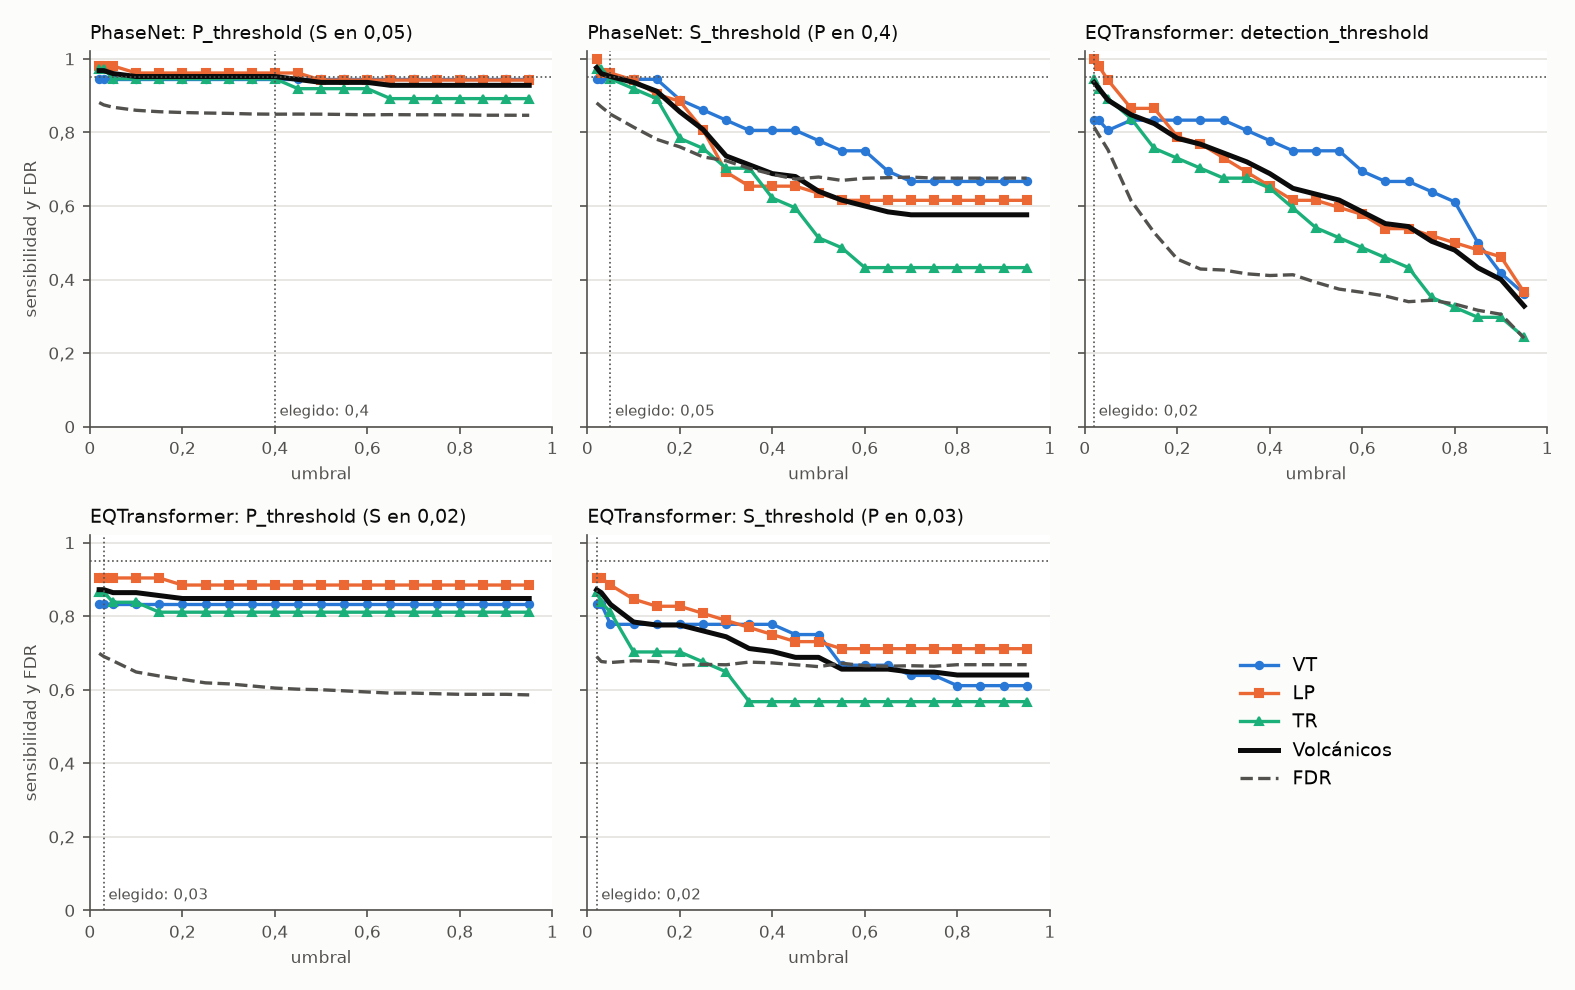
\includegraphics[width=\textwidth]{figuras/fig8_curvas_interseccion.png}
\caption{Sensibilidad por clase, sensibilidad volcánica y FDR según el umbral,
con la intersección y las ventanas de la configuración de cada red.}
\label{fig:res-curvas}
\end{figure}

En PhaseNet, con \texttt{S\_threshold} en 0,05, mover \texttt{P\_threshold}
casi no cambia la sensibilidad, porque la onda S detecta la mayor parte de los
volcánicos. Con \texttt{P\_threshold} en 0,40, en cambio, subir
\texttt{S\_threshold} baja la sensibilidad en todas las clases, y más en TR,
que cae a 0,43 cuando el umbral pasa de 0,60. En EQTransformer ocurre lo mismo
con sus umbrales de P y S. Con su curva de detección, la sensibilidad y la FDR
bajan juntas al subir el umbral.

La Figura~\ref{fig:res-costo} muestra el costo de cada nivel de sensibilidad
en falsas alarmas por hora. Cada punto es una combinación de umbrales con las
ventanas de la configuración de cada red; los puntos grandes son las
configuraciones elegidas, y STA/LTA aparece como un solo punto porque sus
parámetros no se mueven.

\begin{figure}[!ht]
\centering
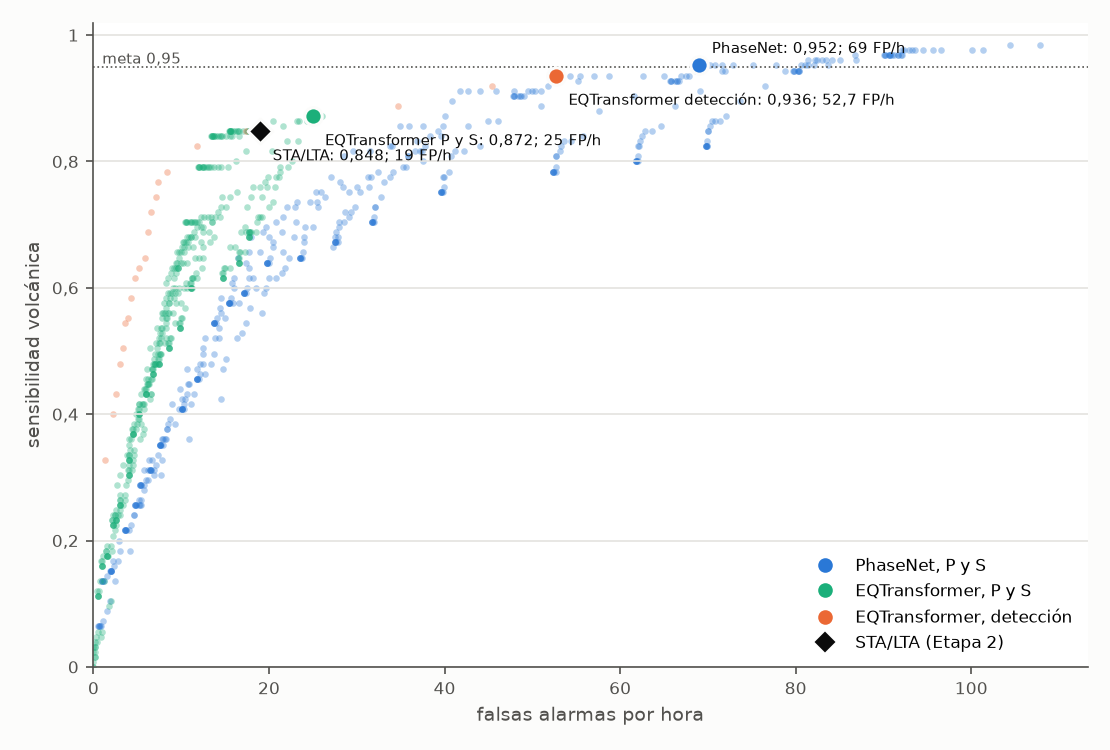
\includegraphics[width=0.85\textwidth]{figuras/fig9_costo_interseccion.png}
\caption{Sensibilidad volcánica contra falsas alarmas por hora. Cada punto es
una combinación de umbrales; los puntos grandes, la configuración elegida de
cada detector.}
\label{fig:res-costo}
\end{figure}

Con menos de 20 falsas alarmas por hora, EQTransformer con P y S y STA/LTA
llegan cerca de 0,85, más que PhaseNet con la misma cantidad de falsas
alarmas. Para pasar de ahí el costo sube rápido: solo PhaseNet supera 0,94, y
para llegar a 0,95 necesita 69,0 falsas alarmas por hora.

\subsection{Qué onda detecta cada evento}

Con \texttt{P\_threshold} en 0,40 y \texttt{S\_threshold} en 0,05, la onda S
sostiene casi toda la detección de PhaseNet: sola detecta 116 volcánicos
(0,928, con 73,3 falsas alarmas por hora), y la P sola, 72 (0,576, con 15,5).
El Cuadro~\ref{tab:res-onda} los separa por clase; ``solo P'' quiere decir que
la P detecta el evento y la S no.

{\small
\setlength{\tabcolsep}{3pt}
\begin{longtable}{lrrrrrrrr}
\caption{Volcánicos según la onda que los detecta, con la configuración de cada
red.}\label{tab:res-onda}\\
\cabecera{ & \multicolumn{4}{c}{\textbf{PhaseNet}} & \multicolumn{4}{c}{\textbf{EQTransformer}} \\ \textbf{Clase} & \textbf{Ambas} & \textbf{Solo P} & \textbf{Solo S} & \textbf{Ninguna} & \textbf{Ambas} & \textbf{Solo P} & \textbf{Solo S} & \textbf{Ninguna}}{9}
VT & 24 & 0 & 10 & 2 & 22 & 0 & 8 & 6 \\
LP & 31 & 1 & 18 & 2 & 36 & 1 & 10 & 5 \\
TR & 14 & 2 & 19 & 2 & 21 & 2 & 9 & 5 \\
\end{longtable}
}

En PhaseNet, la S detecta 47 volcánicos que la P no ve, y la P solo 3 que la S
no ve. Esto tiene un costo en el recorte, que empieza 2,5\,s antes del aviso:
cuando el aviso viene solo de la S, el recorte puede empezar después del
inicio del evento (Sección~\ref{sec:res-recorte}).

\subsection{Las dos redes juntas y las tres componentes}

Se juntaron las dos redes para ver si EQTransformer suma volcánicos que
PhaseNet no detecta. Los intervalos de PhaseNet y los de la curva de detección
de EQTransformer, cada uno con su configuración, se juntaron con la misma
regla que la P y la S: los que empiezan a 5\,s o menos del primero cuentan
como uno. Juntas detectan 122 de 125 volcánicos (0,976): 34 de 36 VT, 52 de 52
LP y 36 de 37 TR, con 101,0 falsas alarmas por hora. Frente a PhaseNet sola,
suman 2 LP y 1 TR, no pierden ninguno y cuestan 32 falsas alarmas por hora
más. El sistema usa solo PhaseNet.

Las dos redes esperan las tres componentes de la estación. Cuando solo se
tiene la vertical, una práctica posible es rellenar N y E con ceros. Con el
criterio anterior de 5\,s y umbral 0,10, esa opción baja a PhaseNet a 0,656 de
los volcánicos, contra 0,904 con Z, N y E reales; copiar la vertical en N y E
da 0,912. En EQTransformer, los ceros dan 0,624 y las tres componentes reales,
0,552. Las dos redes se usan con las tres componentes reales: aunque
EQTransformer rinde algo menos con ellas, así las dos reciben la misma señal.

% =====================================================================
\section{Calidad del recorte}
\label{sec:res-recorte}

El recorte por energía de PhaseNet (Sección~\ref{sec:recorte}) se comparó con
otras formas de delimitar los eventos, todas con la configuración elegida de
cada detector. La primera es el mismo recorte sin el último paso, el corte en
el aviso siguiente. La segunda es una ventana fija de 81,92\,s que empieza
2,5\,s antes del aviso de PhaseNet, el largo con que vienen cortados los
eventos del conjunto publicado por \textcite{espinosacurilem2025dataset}. Las
otras usan como recorte los intervalos que entregan STA/LTA y EQTransformer,
tal como salen de sus librerías y, como referencia, unidos cuando están a
menos de 5\,s uno de otro. Un evento queda bien recortado si su recorte tiene
un IoU de 0,3 o más con él.

{\footnotesize
\setlength{\tabcolsep}{3pt}
\begin{longtable}{>{\raggedright\arraybackslash}p{3.3cm}rrrrrrr}
\caption{Volcánicos bien recortados (IoU de 0,3 o más), IoU medio de esos
eventos, duración mediana de los recortes que tocan un volcánico (s) y
FP/h de la detección.}\label{tab:res-recortes}\\
\cabecera{\textbf{Recorte} & \textbf{VT} & \textbf{LP} & \textbf{TR} & \textbf{Volcánicos} & \textbf{IoU medio} & \textbf{Duración} & \textbf{FP/h}}{8}
PhaseNet + energía con corte & 35/36 & 49/52 & 24/37 & \textbf{108 = 0,864} & 0,68 & 22,0 & 69,0 \\
PhaseNet + energía & 34/36 & 37/52 & 27/37 & 98 = 0,784 & 0,69 & 31,8 & 69,0 \\
PhaseNet + ventana fija de 81,92\,s & 3/36 & 43/52 & 37/37 & 83 = 0,664 & 0,54 & 81,9 & 69,0 \\
STA/LTA, recorte propio & 28/36 & 34/52 & 4/37 & 66 = 0,528 & 0,46 & 11,2 & 19,0 \\
EQTransformer, recorte propio & 8/36 & 9/52 & 14/37 & 31 = 0,248 & 0,47 & 18,4 & 52,7 \\
\midrule
STA/LTA, unido a 5\,s & 28/36 & 34/52 & 6/37 & 68 = 0,544 & 0,46 & 11,5 & 19,0 \\
EQTransformer, unido a 5\,s & 11/36 & 10/52 & 15/37 & 36 = 0,288 & 0,48 & 20,4 & 52,7 \\
\end{longtable}
}

El mejor es el recorte por energía con corte: 108 de 125 volcánicos bien
recortados (0,864). La ventana fija solo gana en TR, porque con 81,92\,s cubre
casi cualquier evento largo; en VT, que duran unos 12\,s, acierta 3 de 36.
STA/LTA pierde casi todos los TR (4 de 37). Los recortes de EQTransformer duran
18,4\,s en mediana, y los eventos, 32,6\,s, así que se quedan cortos: recorta
bien solo 31 volcánicos. Unir los intervalos a 5\,s cambia poco: 2 eventos más
en STA/LTA y 5 en EQTransformer.

El corte en el aviso siguiente se agregó porque, sin él, muchos recortes
salían demasiado largos: con eventos seguidos, el recorte se tragaba al
siguiente (Figura~\ref{fig:res-fallas}, arriba). El corte sube LP de 37 a 49,
pero baja TR de 27 a 24, probablemente porque PhaseNet da varios avisos dentro
de un mismo tremor. Además, con umbral 0,10 se vio que 6 TR quedan cortos
porque en FRE casi no sobresalen del ruido: su energía llega solo a entre 0,8 y
1,6 veces el nivel del ruido (Figura~\ref{fig:res-fallas}, abajo). La
Figura~\ref{fig:res-ejemplos} muestra un caso típico de cada clase.

\begin{figure}[!ht]
\centering
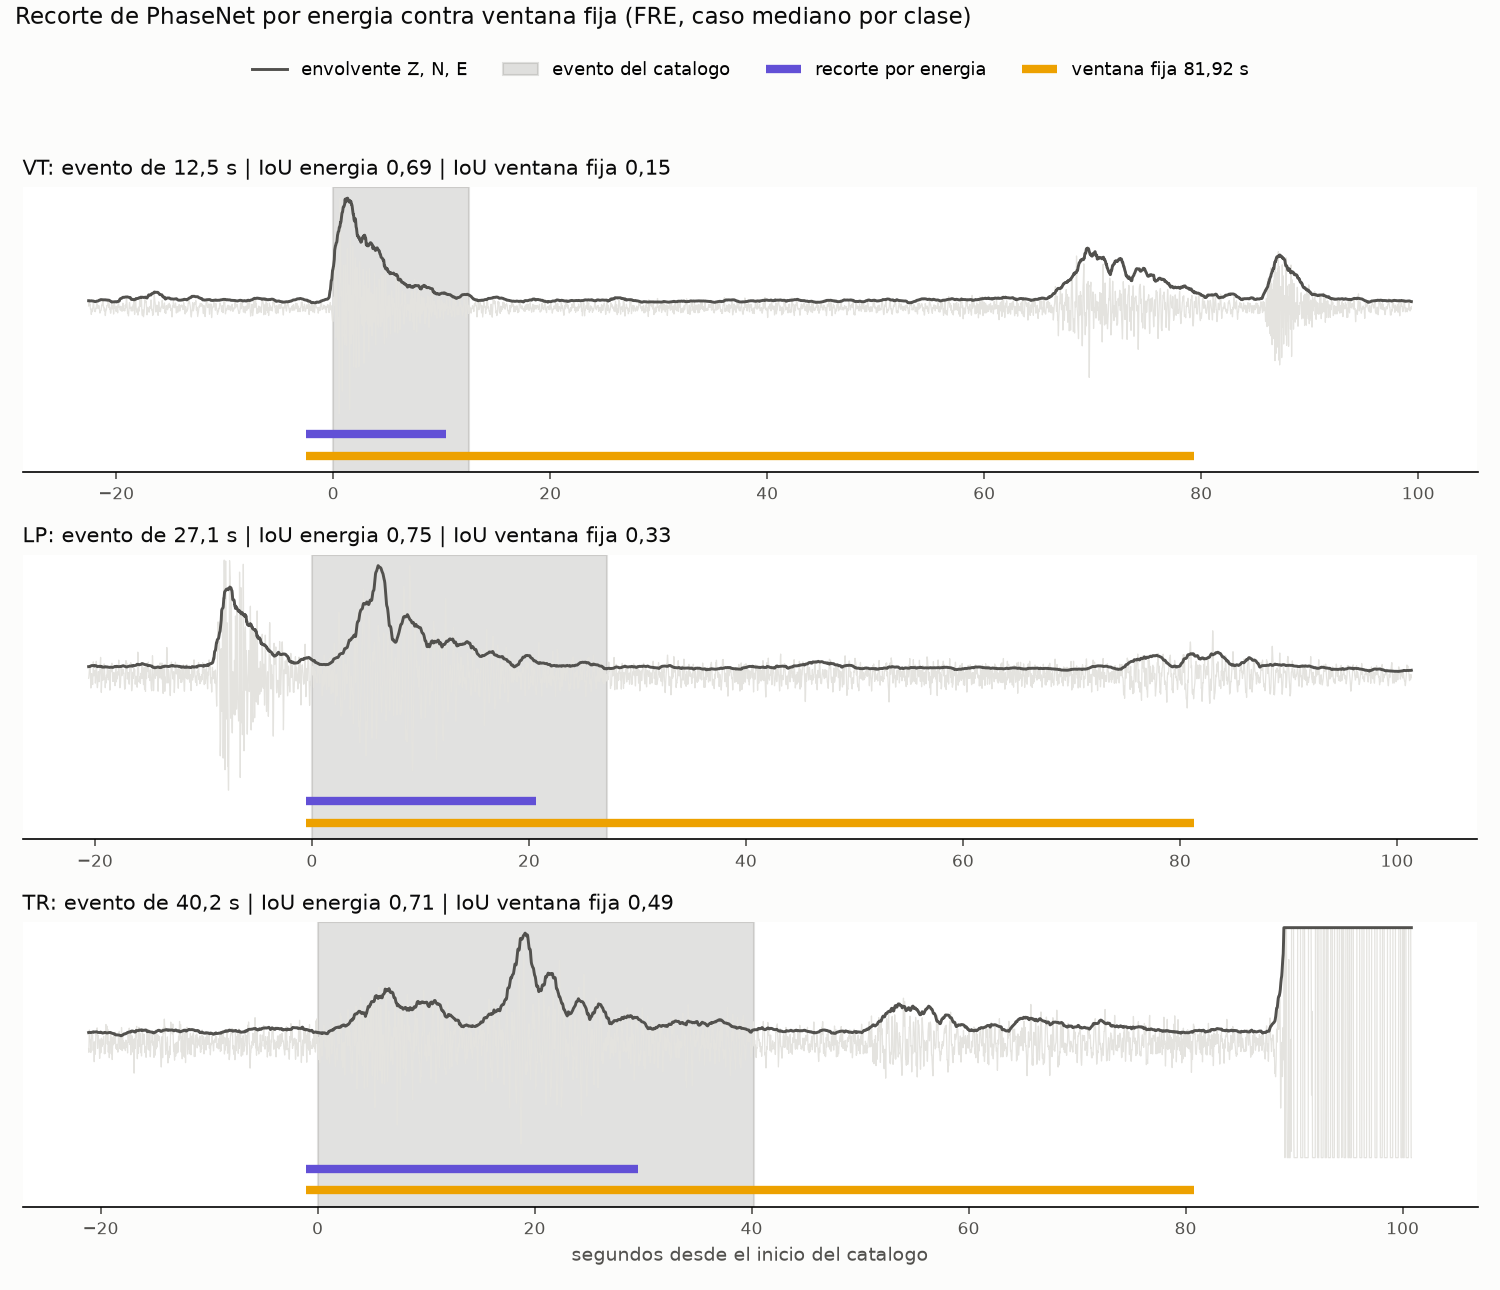
\includegraphics[width=0.78\textwidth]{figuras/fig5_recortes.png}
\caption{Recorte por energía, sin el corte en el aviso siguiente, y ventana
fija en un caso típico de cada clase volcánica, con los avisos de PhaseNet en
umbral 0,10. En el panel de TR, desde los 89\,s aparece una señal mucho mayor
que sale de la escala.}
\label{fig:res-ejemplos}
\end{figure}

\begin{figure}[!ht]
\centering
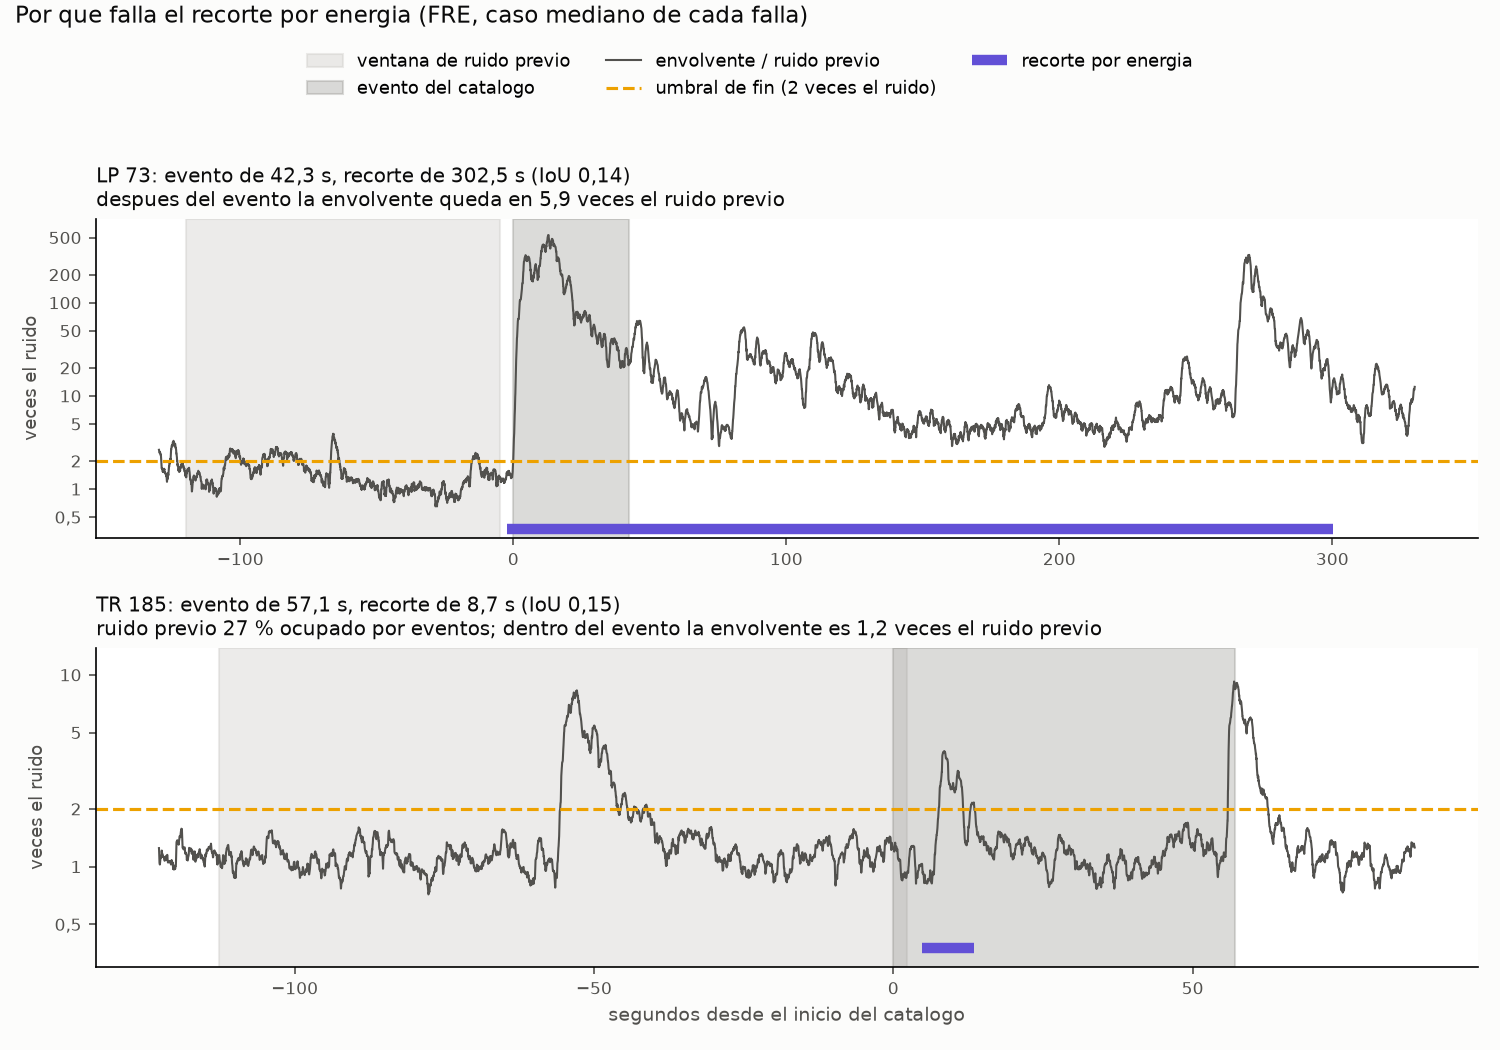
\includegraphics[width=0.80\textwidth]{figuras/fig6_fallas.png}
\caption{Dos fallas del recorte por energía, con los avisos de PhaseNet en
umbral 0,10: un LP con recorte demasiado largo y un TR con recorte demasiado
corto. La energía está medida en veces el ruido previo; el recorte termina
cuando baja de la línea punteada durante 5\,s.}
\label{fig:res-fallas}
\end{figure}

\subsection{Calidad con varios umbrales de IoU}

El umbral de 0,3 es una decisión propia de este trabajo, así que se contó
también cuántos volcánicos tienen un recorte que los toca y cuántos superan
cada umbral de IoU, de 0,1 a 0,9 (Cuadro~\ref{tab:res-iou} y
Figura~\ref{fig:res-iou}).

{\small
\setlength{\tabcolsep}{3pt}
\begin{longtable}{>{\raggedright\arraybackslash}p{5.0cm}rrrrrrrrrr}
\caption{Volcánicos, de 125, con un recorte que los toca y con IoU igual o
mayor que cada umbral.}\label{tab:res-iou}\\
\cabecera{\textbf{Recorte} & \textbf{Toca} & \textbf{0,1} & \textbf{0,2} & \textbf{0,3} & \textbf{0,4} & \textbf{0,5} & \textbf{0,6} & \textbf{0,7} & \textbf{0,8} & \textbf{0,9}}{11}
PhaseNet + energía con corte & 122 & 120 & 112 & 108 & 102 & 87 & 69 & 49 & 32 & 14 \\
PhaseNet + energía & 120 & 120 & 105 & 98 & 94 & 83 & 69 & 49 & 29 & 13 \\
PhaseNet + ventana fija de 81,92\,s & 125 & 124 & 101 & 83 & 60 & 39 & 22 & 17 & 10 & 5 \\
EQTransformer, recorte propio & 117 & 105 & 68 & 31 & 18 & 10 & 5 & 4 & 1 & 0 \\
STA/LTA, recorte propio & 106 & 100 & 90 & 66 & 39 & 20 & 14 & 5 & 2 & 0 \\
\end{longtable}
}

\begin{figure}[!ht]
\centering
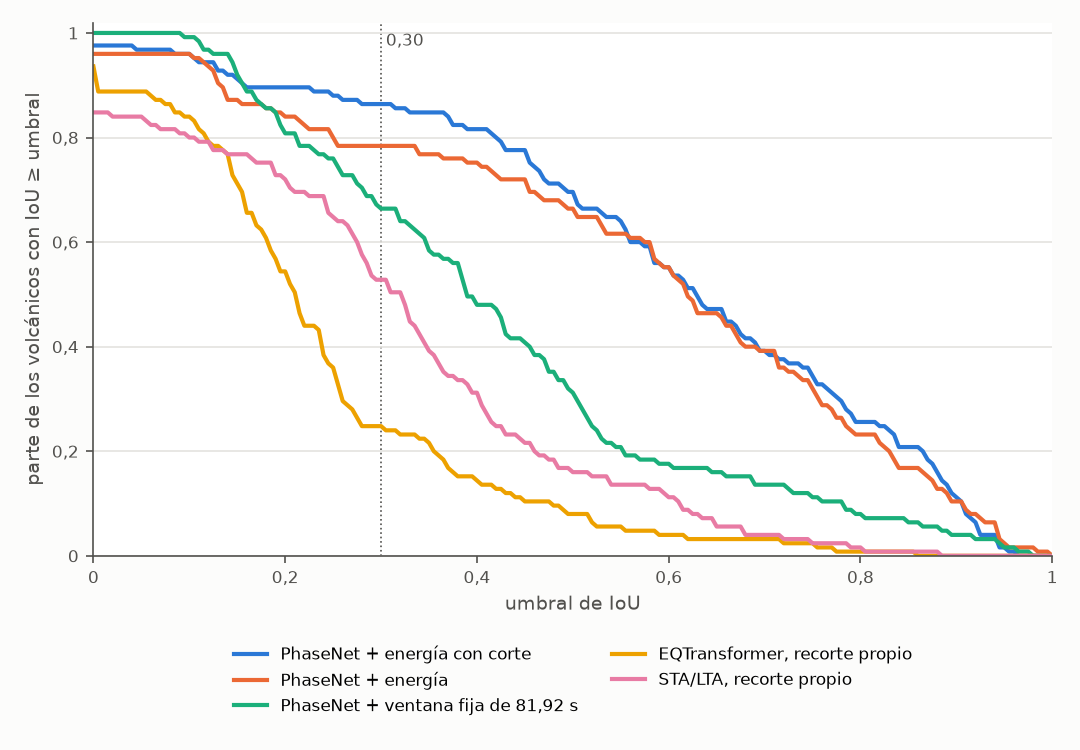
\includegraphics[width=0.80\textwidth]{figuras/fig7_iou.png}
\caption{Parte de los 125 volcánicos con IoU igual o mayor que cada umbral,
para cada recorte. La línea punteada marca el umbral de 0,3.}
\label{fig:res-iou}
\end{figure}

Tocar el evento no basta. Si se cuenta todo recorte que lo toca, el recorte
por energía con corte llega a 122 de 125 (0,976) y la ventana fija toca los
125, pero los toca porque es larga: en VT su IoU mediano es 0,19. Con IoU de
0,5 o más, el recorte por energía con corte delimita bien 87 volcánicos
(0,696); sin corte, 83; la ventana fija, 39; STA/LTA, 20, y EQTransformer, 10.
El Cuadro~\ref{tab:res-iou-clase} separa por clase.

{\small
\setlength{\tabcolsep}{4pt}
\begin{longtable}{>{\raggedright\arraybackslash}p{5.0cm}lrrrrr}
\caption{Por clase: eventos con un recorte que los toca y con IoU de 0,3, 0,5
y 0,7 o más, e IoU mediano de los que se tocan.}\label{tab:res-iou-clase}\\
\cabecera{\textbf{Recorte} & \textbf{Clase} & \textbf{Toca} & \textbf{0,3} & \textbf{0,5} & \textbf{0,7} & \textbf{Mediana}}{7}
PhaseNet + energía con corte & VT (36) & 35 & 35 & 33 & 18 & 0,71 \\
 & LP (52) & 51 & 49 & 40 & 24 & 0,67 \\
 & TR (37) & 36 & 24 & 14 & 7 & 0,44 \\
\midrule
PhaseNet + energía & VT (36) & 35 & 34 & 32 & 17 & 0,69 \\
 & LP (52) & 50 & 37 & 28 & 18 & 0,56 \\
 & TR (37) & 35 & 27 & 23 & 14 & 0,62 \\
\midrule
PhaseNet + ventana fija de 81,92\,s & VT (36) & 36 & 3 & 0 & 0 & 0,19 \\
 & LP (52) & 52 & 43 & 13 & 0 & 0,41 \\
 & TR (37) & 37 & 37 & 26 & 17 & 0,69 \\
\midrule
EQTransformer, recorte propio & VT (36) & 30 & 8 & 0 & 0 & 0,24 \\
 & LP (52) & 52 & 9 & 2 & 0 & 0,20 \\
 & TR (37) & 35 & 14 & 8 & 4 & 0,26 \\
\midrule
STA/LTA, recorte propio & VT (36) & 32 & 28 & 13 & 4 & 0,46 \\
 & LP (52) & 45 & 34 & 5 & 1 & 0,36 \\
 & TR (37) & 29 & 4 & 2 & 0 & 0,19 \\
\end{longtable}
}

Con el recorte por energía con corte, VT y LP quedan bien delimitados (IoU
mediano de 0,71 y 0,67) y TR es lo más débil (0,44). En TR rinden mejor el
mismo recorte sin corte (0,62) y la ventana fija (0,69), porque el tremor es
largo.

\subsection{Cómo falla el recorte}

Cuando un recorte toca su evento, puede hacerlo de cuatro formas: cubrirlo
entero, empezando antes y terminando después; empezar antes y terminar dentro
del evento, de modo que le falta el final; quedar dentro del evento, de modo
que le faltan el inicio y el fin; o empezar dentro del evento y terminar
después, de modo que le falta el inicio. El Cuadro~\ref{tab:res-casos} cuenta
cuántos volcánicos caen en cada caso; cada fila suma 125.

{\footnotesize
\setlength{\tabcolsep}{3pt}
\begin{longtable}{>{\raggedright\arraybackslash}p{3.0cm}>{\raggedleft\arraybackslash}p{1.8cm}>{\raggedleft\arraybackslash}p{1.8cm}>{\raggedleft\arraybackslash}p{1.8cm}>{\raggedleft\arraybackslash}p{1.8cm}>{\raggedleft\arraybackslash}p{1.8cm}}
\caption{Volcánicos según cómo los toca su recorte; entre paréntesis, IoU
mediano.}\label{tab:res-casos}\\
\cabecera{\textbf{Recorte} & \textbf{Cubre todo} & \textbf{Falta el final} & \textbf{Faltan inicio y fin} & \textbf{Falta el inicio} & \textbf{No lo toca}}{6}
PhaseNet + energía con corte & 26 (0,72) & 46 (0,71) & 36 (0,53) & 14 (0,68) & 3 \\
PhaseNet + energía & 37 (0,53) & 40 (0,74) & 20 (0,60) & 23 (0,62) & 5 \\
PhaseNet + ventana fija de 81,92\,s & 91 (0,34) & 5 (0,64) & 17 (0,66) & 12 (0,53) & 0 \\
EQTransformer, recorte propio & 5 (0,49) & 65 (0,24) & 40 (0,17) & 7 (0,43) & 8 \\
STA/LTA, recorte propio & 0 & 13 (0,40) & 92 (0,33) & 1 (0,52) & 19 \\
\end{longtable}
}

El recorte por energía con corte falla sobre todo por el final: en 82
volcánicos termina antes que el evento (46 más 36), y en 50 empieza después
del inicio que marca el catálogo (36 más 14). STA/LTA corta corto: en 92 casos
su recorte queda dentro del evento. EQTransformer suele empezar antes del
evento y terminar antes de su fin.

Que el recorte empiece tarde depende de qué onda dio el aviso. Como la onda S
llega después de la P, cuando PhaseNet solo ve la S el margen de 2,5\,s puede
no alcanzar. El Cuadro~\ref{tab:res-inicio} lo mide para cada volcánico que su
recorte toca.

{\small
\setlength{\tabcolsep}{4pt}
\begin{longtable}{llr>{\raggedleft\arraybackslash}p{1.7cm}>{\raggedleft\arraybackslash}p{1.9cm}>{\raggedleft\arraybackslash}p{2.8cm}>{\raggedleft\arraybackslash}p{1.7cm}}
\caption{Inicio del recorte por energía con corte según la onda que dio el
aviso.}\label{tab:res-inicio}\\
\cabecera{\textbf{Onda} & \textbf{Clase} & \textbf{Eventos} & \textbf{Empieza antes} & \textbf{Empieza después} & \textbf{Aviso tras el inicio, mediana (s)} & \textbf{IoU mediano}}{7}
P & VT & 28 & 23 & 5 & 1,5 & 0,73 \\
P & LP & 35 & 26 & 9 & 1,6 & 0,69 \\
P & TR & 7 & 6 & 1 & 0,8 & 0,50 \\
P & Todas & 70 & 55 & 15 & 1,6 & 0,72 \\
\midrule
S & VT & 7 & 6 & 1 & 0,0 & 0,61 \\
S & LP & 16 & 7 & 9 & 2,8 & 0,64 \\
S & TR & 29 & 4 & 25 & 12,9 & 0,42 \\
S & Todas & 52 & 17 & 35 & 4,4 & 0,55 \\
\end{longtable}
}

Cuando avisa la P, el recorte empieza antes del inicio en 55 de 70 casos: el
aviso llega en mediana 1,6\,s después del inicio, dentro del margen de 2,5\,s.
Cuando el aviso viene de la S, el recorte empieza después del inicio en 35 de 52
casos, porque la S llega en mediana 4,4\,s después; en esos casos el recorte
pierde la onda P. Casi todos son TR: en 25 de los 29 TR avisados por la S, el
recorte empieza tarde, con el aviso 12,9\,s después del inicio en
mediana. Bajar \texttt{P\_threshold} casi no lo corrige: con 0,02, en 4 de los
21 recortes que empezaban tarde con 0,10 para las dos ondas el aviso pasa a
venir de la P, pero solo 1 empieza antes del inicio. En estos eventos, casi
todos TR, PhaseNet no marca una onda P temprana ni con umbrales muy bajos.

% =====================================================================
\section{Detección y recorte en las ventanas de test}
\label{sec:res-deteccion-test}

La misma detección y el mismo recorte, con la configuración elegida, se
aplicaron a las 1.161 ventanas de test, que no se usaron para elegir ningún
parámetro. Cada ventana tiene su evento principal al centro, así que se cuenta
cuántos de esos eventos se detectan y cuántos quedan con un recorte de IoU de
0,3 o más (Cuadro~\ref{tab:res-test-deteccion}).

\needspace{9\baselineskip}
{\footnotesize
\setlength{\tabcolsep}{3pt}
\begin{longtable}{lrrlrl}
\caption{Detección y recorte del evento principal de las ventanas de test.
Entre corchetes, el intervalo de confianza del 95\,\%.}\label{tab:res-test-deteccion}\\
\cabecera{\textbf{Clase} & \textbf{Eventos} & \textbf{Detectados} & \textbf{Sensibilidad} & \textbf{IoU $\geq$ 0,3} & \textbf{Parte}}{6}
VT & 300 & 300 & 1,000 [0,987; 1,000] & 293 & 0,977 [0,953; 0,989] \\
LP & 288 & 278 & 0,965 [0,937; 0,981] & 281 & 0,976 [0,951; 0,988] \\
TR & 281 & 267 & 0,950 [0,918; 0,970] & 183 & 0,651 [0,594; 0,705] \\
\midrule
\textbf{Volcánicos} & \textbf{869} & \textbf{845} & \textbf{0,972 [0,959; 0,981]} & \textbf{757} & \textbf{0,871 [0,847; 0,892]} \\
\end{longtable}
}

La sensibilidad de detección y la parte bien recortada son parecidas a las de
la traza continua (0,972 contra 0,952 y 0,871 contra 0,864), y en las dos TR es
la clase peor recortada: 0,651 en test y 24 de 37 (0,649) en la traza. En LP
hay más eventos bien recortados (281) que detectados (278), porque la
detección se cuenta con los intervalos de los avisos, que son cortos, y el
recorte, que es más largo, puede tocar un evento cuyo aviso no lo tocó.

En las 1.161 ventanas, que suman 96,75 horas, la detección y el recorte
producen 7.621 recortes, 6,6 por ventana. Los que no quedan emparejados con
ninguna caja del catálogo son 59,5 por hora, el 75,6\,\% de todos los recortes.
Detectar y recortar una ventana de 300\,s toma 0,02\,s en el procesador del
computador, sin tarjeta gráfica.

% =====================================================================
\section{Clasificador}
\label{sec:res-clasificador}

\subsection{Búsqueda de la configuración}
\label{subsec:res-busqueda}

La búsqueda hizo 20 pruebas por red, entrenando con los folds 2 a 5 y
validando con el fold 1 (Sección~\ref{subsec:busqueda}). El
Cuadro~\ref{tab:res-busqueda} muestra la combinación con mayor F1 macro de VT,
LP y TR en validación para cada red.

{\small
\setlength{\tabcolsep}{4pt}
\begin{longtable}{>{\raggedright\arraybackslash}p{3.2cm}>{\raggedright\arraybackslash}p{3.0cm}>{\raggedright\arraybackslash}p{3.0cm}>{\raggedright\arraybackslash}p{3.0cm}}
\caption{Mejor combinación de cada red en la búsqueda (fold 1 de
validación).}\label{tab:res-busqueda}\\
\cabecera{\textbf{Parámetro} & \textbf{EfficientNet-B0} & \textbf{ResNet50} & \textbf{VGG16}}{4}
Optimizador & AdamW & SGD con momentum 0,9 & AdamW \\
Tasa de aprendizaje & 0,001 & 0,01 & 0,00001 \\
Dropout & 0,3 & 0,3 & 0,3 \\
Tamaño de lote & 16 & 32 & 16 \\
Weight decay & 0 & 0 & 0,0001 \\
Función de pérdida & Focal & Entropía cruzada con pesos & Entropía cruzada con pesos \\
\midrule
F1 macro de VT, LP y TR en validación & 0,866 & 0,859 & 0,856 \\
\end{longtable}
}

Las tres redes quedan con dropout 0,3, el mayor de los dos probados, y cada una
con una tasa de aprendizaje distinta. Entre la mejor y la peor hay 0,010 de F1
macro, menos que la variación entre folds de una misma red que se ve más
adelante.

Para ver cuánto aportan la búsqueda, el aumento de datos y la parada temprana,
el Cuadro~\ref{tab:res-antes} compara cada red, en el mismo fold de
validación, con una configuración inicial sin ellos: AdamW con tasa de
aprendizaje 0,0001, 10 épocas y sin aumento de datos.

\needspace{9\baselineskip}
{\small
\begin{longtable}{lrrr}
\caption{F1 macro de VT, LP y TR en el fold 1 de validación, con la
configuración inicial y con la elegida.}\label{tab:res-antes}\\
\cabecera{\textbf{Red} & \textbf{Inicial} & \textbf{Elegida} & \textbf{Diferencia}}{4}
EfficientNet-B0 & 0,834 & 0,866 & +0,032 \\
ResNet50 & 0,835 & 0,859 & +0,024 \\
VGG16 & 0,835 & 0,856 & +0,021 \\
\end{longtable}
}

La mejora es de 0,02 a 0,03 en las tres redes. Por clase, la sensibilidad de
VT sube de entre 0,89 y 0,92 a entre 0,92 y 0,95, y la de TR queda parecida
(de entre 0,78 y 0,81 a entre 0,75 y 0,82). Como se mide en una sola partición,
la mejora es del mismo orden que la variación entre folds.

\subsection{Validación cruzada y test}
\label{subsec:res-folds}

Con la combinación elegida, cada red se entrenó cinco veces, una por fold de
validación, y el mejor modelo de cada vez se evaluó en las 1.161 ventanas de
test. En test hay 336 recortes VT, 676 LP, 244 TR y 320 de rechazo con IoU de
0,3 o más y 5\,s o más de duración. El Cuadro~\ref{tab:res-f1} resume el F1 macro de VT, LP y TR de los
cinco modelos, con el recorte y con la ventana fija de 60\,s.

\needspace{9\baselineskip}
{\small
\setlength{\tabcolsep}{4pt}
\begin{longtable}{>{\raggedright\arraybackslash}p{2.6cm}>{\raggedright\arraybackslash}p{2.0cm}>{\raggedright\arraybackslash}p{3.2cm}>{\raggedright\arraybackslash}p{3.2cm}}
\caption{F1 macro de VT, LP y TR de los cinco modelos de cada red: promedio
y desviación estándar y, debajo, mínimo y máximo entre corchetes.}\label{tab:res-f1}\\
\cabecera{\textbf{Red} & \textbf{Entrada} & \textbf{Validación} & \textbf{Test}}{4}
EfficientNet-B0 & Recorte & 0,871 $\pm$ 0,007 \newline [0,864; 0,880] & 0,840 $\pm$ 0,009 \newline [0,828; 0,848] \\
 & Fija de 60\,s & 0,862 $\pm$ 0,013 \newline [0,846; 0,877] & 0,835 $\pm$ 0,006 \newline [0,828; 0,844] \\
\midrule
ResNet50 & Recorte & 0,865 $\pm$ 0,007 \newline [0,859; 0,876] & 0,834 $\pm$ 0,012 \newline [0,823; 0,853] \\
 & Fija de 60\,s & 0,860 $\pm$ 0,014 \newline [0,842; 0,879] & 0,831 $\pm$ 0,003 \newline [0,826; 0,835] \\
\midrule
VGG16 & Recorte & 0,866 $\pm$ 0,014 \newline [0,856; 0,891] & 0,843 $\pm$ 0,008 \newline [0,833; 0,853] \\
 & Fija de 60\,s & 0,855 $\pm$ 0,008 \newline [0,843; 0,861] & 0,834 $\pm$ 0,009 \newline [0,825; 0,847] \\
\end{longtable}
}

En test, el F1 macro con el recorte va de 0,834 a 0,843 según la red, entre
0,02 y 0,03 menos que en validación. Esa diferencia es esperable, porque la
validación se usa para elegir la época y, en el fold 1, la configuración. Las
diferencias entre redes, de hasta 0,009, son menores que la distancia entre
el mejor y el peor de los cinco modelos de una misma red, que llega a 0,030;
con estos datos ninguna de las tres redes supera claramente a las otras. La
ventana fija de 60\,s queda entre 0,831 y 0,835.

Los Cuadros~\ref{tab:res-clases-recorte} y~\ref{tab:res-clases-fija} separan
por clase la sensibilidad y el F1 en test.

{\small
\setlength{\tabcolsep}{4pt}
\begin{longtable}{>{\raggedright\arraybackslash}p{2.0cm}>{\raggedright\arraybackslash}p{3.4cm}>{\raggedright\arraybackslash}p{3.4cm}>{\raggedright\arraybackslash}p{3.4cm}}
\caption{Test con el recorte: sensibilidad por clase, con mínimo y máximo de
los cinco modelos entre corchetes, y F1 promedio.}\label{tab:res-clases-recorte}\\
\cabecera{\textbf{Clase} & \textbf{EfficientNet-B0} & \textbf{ResNet50} & \textbf{VGG16}}{4}
\multicolumn{4}{l}{\textit{Sensibilidad}}\\*
VT & 0,893 [0,875; 0,908] & 0,910 [0,881; 0,949] & 0,889 [0,854; 0,920] \\
LP & 0,869 [0,837; 0,895] & 0,812 [0,780; 0,870] & 0,834 [0,812; 0,852] \\
TR & 0,764 [0,734; 0,840] & 0,831 [0,787; 0,877] & 0,811 [0,803; 0,824] \\
Rechazo & 0,853 [0,791; 0,916] & 0,857 [0,769; 0,909] & 0,904 [0,875; 0,928] \\
\midrule
\multicolumn{4}{l}{\textit{F1}}\\*
VT & 0,854 & 0,841 & 0,848 \\
LP & 0,872 & 0,855 & 0,867 \\
TR & 0,794 & 0,805 & 0,815 \\
Rechazo & 0,861 & 0,861 & 0,875 \\
\end{longtable}
}

{\small
\setlength{\tabcolsep}{4pt}
\begin{longtable}{>{\raggedright\arraybackslash}p{2.0cm}>{\raggedright\arraybackslash}p{3.4cm}>{\raggedright\arraybackslash}p{3.4cm}>{\raggedright\arraybackslash}p{3.4cm}}
\caption{Test con la ventana fija de 60\,s: sensibilidad por clase, con mínimo
y máximo de los cinco modelos entre corchetes, y F1 promedio.}\label{tab:res-clases-fija}\\
\cabecera{\textbf{Clase} & \textbf{EfficientNet-B0} & \textbf{ResNet50} & \textbf{VGG16}}{4}
\multicolumn{4}{l}{\textit{Sensibilidad}}\\*
VT & 0,907 [0,860; 0,940] & 0,901 [0,866; 0,932] & 0,900 [0,884; 0,926] \\
LP & 0,856 [0,818; 0,889] & 0,824 [0,808; 0,836] & 0,843 [0,780; 0,892] \\
TR & 0,761 [0,721; 0,803] & 0,777 [0,738; 0,807] & 0,782 [0,742; 0,844] \\
Rechazo & 0,831 [0,766; 0,884] & 0,880 [0,816; 0,916] & 0,855 [0,828; 0,888] \\
\midrule
\multicolumn{4}{l}{\textit{F1}}\\*
VT & 0,849 & 0,846 & 0,854 \\
LP & 0,860 & 0,854 & 0,860 \\
TR & 0,795 & 0,792 & 0,787 \\
Rechazo & 0,856 & 0,862 & 0,862 \\
\end{longtable}
}

VT es la clase que mejor se reconoce en las tres redes, con sensibilidades
entre 0,889 y 0,910 con el recorte. TR es la más difícil: entre 0,764 y 0,831.
La Figura~\ref{fig:res-matrices-test} muestra con qué se confunde cada clase.
TR va a LP entre el 13 y el 21\,\% de las veces con el recorte, y del rechazo
entre el 6 y el 10\,\% va a VT. VT y TR casi nunca se confunden entre sí: menos
del 1\,\% en cualquier sentido.

\begin{figure}[!ht]
\centering
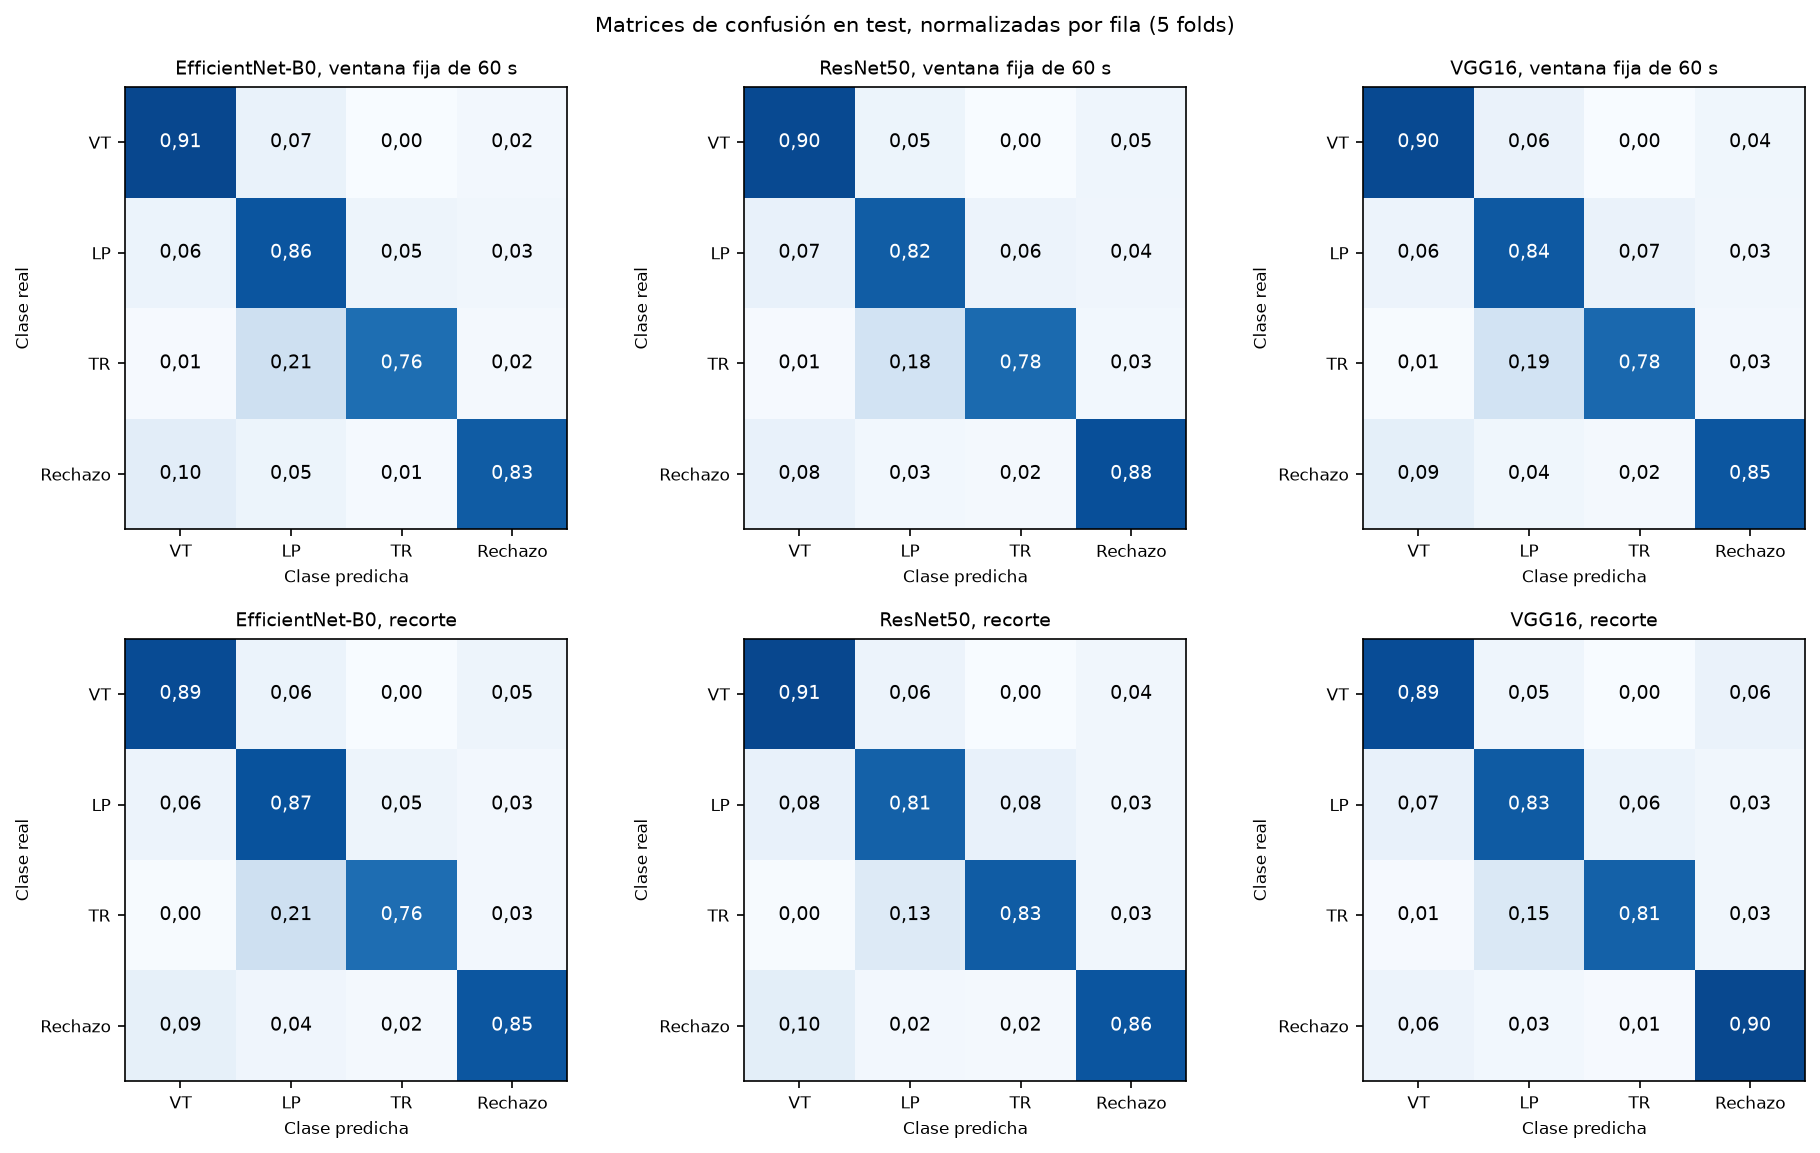
\includegraphics[width=\textwidth]{images/matrices_test.png}
\caption{Matrices de confusión en test, normalizadas por fila (suma de los
cinco modelos de cada red). Arriba, con la ventana fija de 60\,s; abajo, con el
recorte.}
\label{fig:res-matrices-test}
\end{figure}

Los recortes sin caja no se usan para entrenar ni en las métricas anteriores,
pero se clasifican igual, porque en operación el sistema los recibe. En test
hay 2.420 recortes sin caja de 5\,s o más. Con el recorte, EfficientNet-B0
clasifica como volcánicos al 75,0\,\%, ResNet50 al 76,1\,\% y VGG16 al
74,7\,\%; con la ventana fija, al 78,3, 65,8 y 74,7\,\%. El clasificador, que
solo aprendió a separar VT, LP y TR de AV e IC, manda a la clase de rechazo
entre una cuarta y una tercera parte de estos recortes.

% =====================================================================
\section{Sistema completo sobre la traza continua}
\label{sec:res-sistema}

La cadena completa se aplicó a las 9,74 horas válidas de la traza continua de
FRE, con los cinco modelos de cada red. La detección y el recorte dan 1.155
recortes, que se etiquetan contra el catálogo con la misma regla que los de las
ventanas etiquetadas (Cuadro~\ref{tab:res-traza-etiquetas}).

{\small
\begin{longtable}{lr}
\caption{Recortes de la traza continua por etiqueta.}\label{tab:res-traza-etiquetas}\\
\cabecera{\textbf{Etiqueta} & \textbf{Recortes}}{2}
VT & 35 \\
LP & 50 \\
TR & 24 \\
AV & 6 \\
IC & 34 \\
Fuera (tocan un evento con IoU menor que 0,3) & 151 \\
Sin caja (no tocan ningún evento) & 855 \\
\midrule
Total & 1.155 \\
\end{longtable}
}

\subsection{Clasificación y sensibilidad completa}
\label{subsec:res-sistema-clases}

Los 109 recortes volcánicos con IoU de 0,3 o más corresponden a 35 de los 36
VT, 50 de los 52 LP y 24 de los 37 TR. Eso pone un techo a la sensibilidad
completa, la parte de los eventos que el sistema detecta, recorta y clasifica
bien a la vez: aunque el clasificador acertara todos los recortes, el sistema
llegaría a 0,972 en VT, 0,962 en LP, 0,649 en TR y 0,872 en los volcánicos.
El Cuadro~\ref{tab:res-sistema} da los resultados con el recorte y el
Cuadro~\ref{tab:res-sistema-fija}, con la ventana fija de 60\,s. Cada cifra
es el promedio de los cinco modelos de cada red; junto al F1 macro y a la
sensibilidad completa volcánica va la desviación estándar.

{\small
\setlength{\tabcolsep}{4pt}
\begin{longtable}{>{\raggedright\arraybackslash}p{4.0cm}>{\raggedright\arraybackslash}p{2.7cm}>{\raggedright\arraybackslash}p{2.7cm}>{\raggedright\arraybackslash}p{2.7cm}}
\caption{Sistema completo en la traza continua, con el recorte. Entre
paréntesis, cuántos recortes o eventos entran en cada cifra.}\label{tab:res-sistema}\\
\cabecera{\textbf{Medida} & \textbf{EfficientNet-B0} & \textbf{ResNet50} & \textbf{VGG16}}{4}
\multicolumn{4}{l}{\textit{Clasificación de los recortes con IoU de 0,3 o más}}\\*
F1 macro de VT, LP y TR & 0,717 $\pm$ 0,023 & 0,770 $\pm$ 0,029 & 0,719 $\pm$ 0,037 \\
Sensibilidad VT (35) & 0,594 & 0,691 & 0,583 \\
Sensibilidad LP (50) & 0,932 & 0,892 & 0,872 \\
Sensibilidad TR (24) & 0,667 & 0,800 & 0,700 \\
Sensibilidad rechazo (40) & 0,465 & 0,540 & 0,595 \\
\midrule
\multicolumn{4}{l}{\textit{Sensibilidad completa}}\\*
VT (36) & 0,578 & 0,672 & 0,567 \\
LP (52) & 0,896 & 0,858 & 0,838 \\
TR (37) & 0,432 & 0,519 & 0,454 \\
Volcánicos (125) & 0,667 $\pm$ 0,012 & 0,704 $\pm$ 0,020 & 0,646 $\pm$ 0,031 \\
AV (6) & 0,533 & 0,467 & 0,400 \\
IC (48) & 0,321 & 0,392 & 0,446 \\
\midrule
Recortes sin caja clasificados como volcánicos, por hora & 67,9 & 64,5 & 60,0 \\
\end{longtable}
}

{\small
\setlength{\tabcolsep}{4pt}
\begin{longtable}{>{\raggedright\arraybackslash}p{4.0cm}>{\raggedright\arraybackslash}p{2.7cm}>{\raggedright\arraybackslash}p{2.7cm}>{\raggedright\arraybackslash}p{2.7cm}}
\caption{Sistema completo en la traza continua, con la ventana fija de
60\,s.}\label{tab:res-sistema-fija}\\
\cabecera{\textbf{Medida} & \textbf{EfficientNet-B0} & \textbf{ResNet50} & \textbf{VGG16}}{4}
\multicolumn{4}{l}{\textit{Clasificación de los recortes con IoU de 0,3 o más}}\\*
F1 macro de VT, LP y TR & 0,710 $\pm$ 0,028 & 0,708 $\pm$ 0,038 & 0,720 $\pm$ 0,013 \\
Sensibilidad VT (35) & 0,680 & 0,680 & 0,743 \\
Sensibilidad LP (50) & 0,904 & 0,836 & 0,860 \\
Sensibilidad TR (24) & 0,625 & 0,642 & 0,642 \\
Sensibilidad rechazo (40) & 0,470 & 0,600 & 0,510 \\
\midrule
\multicolumn{4}{l}{\textit{Sensibilidad completa}}\\*
VT (36) & 0,661 & 0,661 & 0,722 \\
LP (52) & 0,869 & 0,804 & 0,827 \\
TR (37) & 0,405 & 0,416 & 0,416 \\
Volcánicos (125) & 0,672 $\pm$ 0,020 & 0,648 $\pm$ 0,032 & 0,675 $\pm$ 0,009 \\
AV (6) & 0,467 & 0,767 & 0,567 \\
IC (48) & 0,333 & 0,404 & 0,354 \\
\midrule
Recortes sin caja clasificados como volcánicos, por hora & 65,5 & 52,0 & 64,2 \\
\end{longtable}
}

Con el recorte, la sensibilidad completa volcánica queda entre 0,646 y 0,704
según la red, y el F1 macro de clasificación entre 0,717 y 0,770, contra 0,834
a 0,843 en test. LP es la clase que mejor se sostiene (0,838 a 0,896 de
sensibilidad completa). En TR, la mayor parte de la pérdida viene del recorte:
el techo es 0,649 y la clasificación de los 24 recortes que calzan acierta
entre 0,667 y 0,800. En VT ocurre lo contrario: casi todos quedan bien
recortados, pero la clasificación acierta entre 0,583 y 0,691. La
Figura~\ref{fig:res-matrices-traza} muestra a dónde van: con el recorte, entre
el 14 y el 24\,\% de los VT se clasifica como LP y entre el 16 y el 27\,\%
como rechazo. Del rechazo, el 26\,\% va a VT y entre el 14 y el 27\,\%, a LP.

\begin{figure}[!ht]
\centering
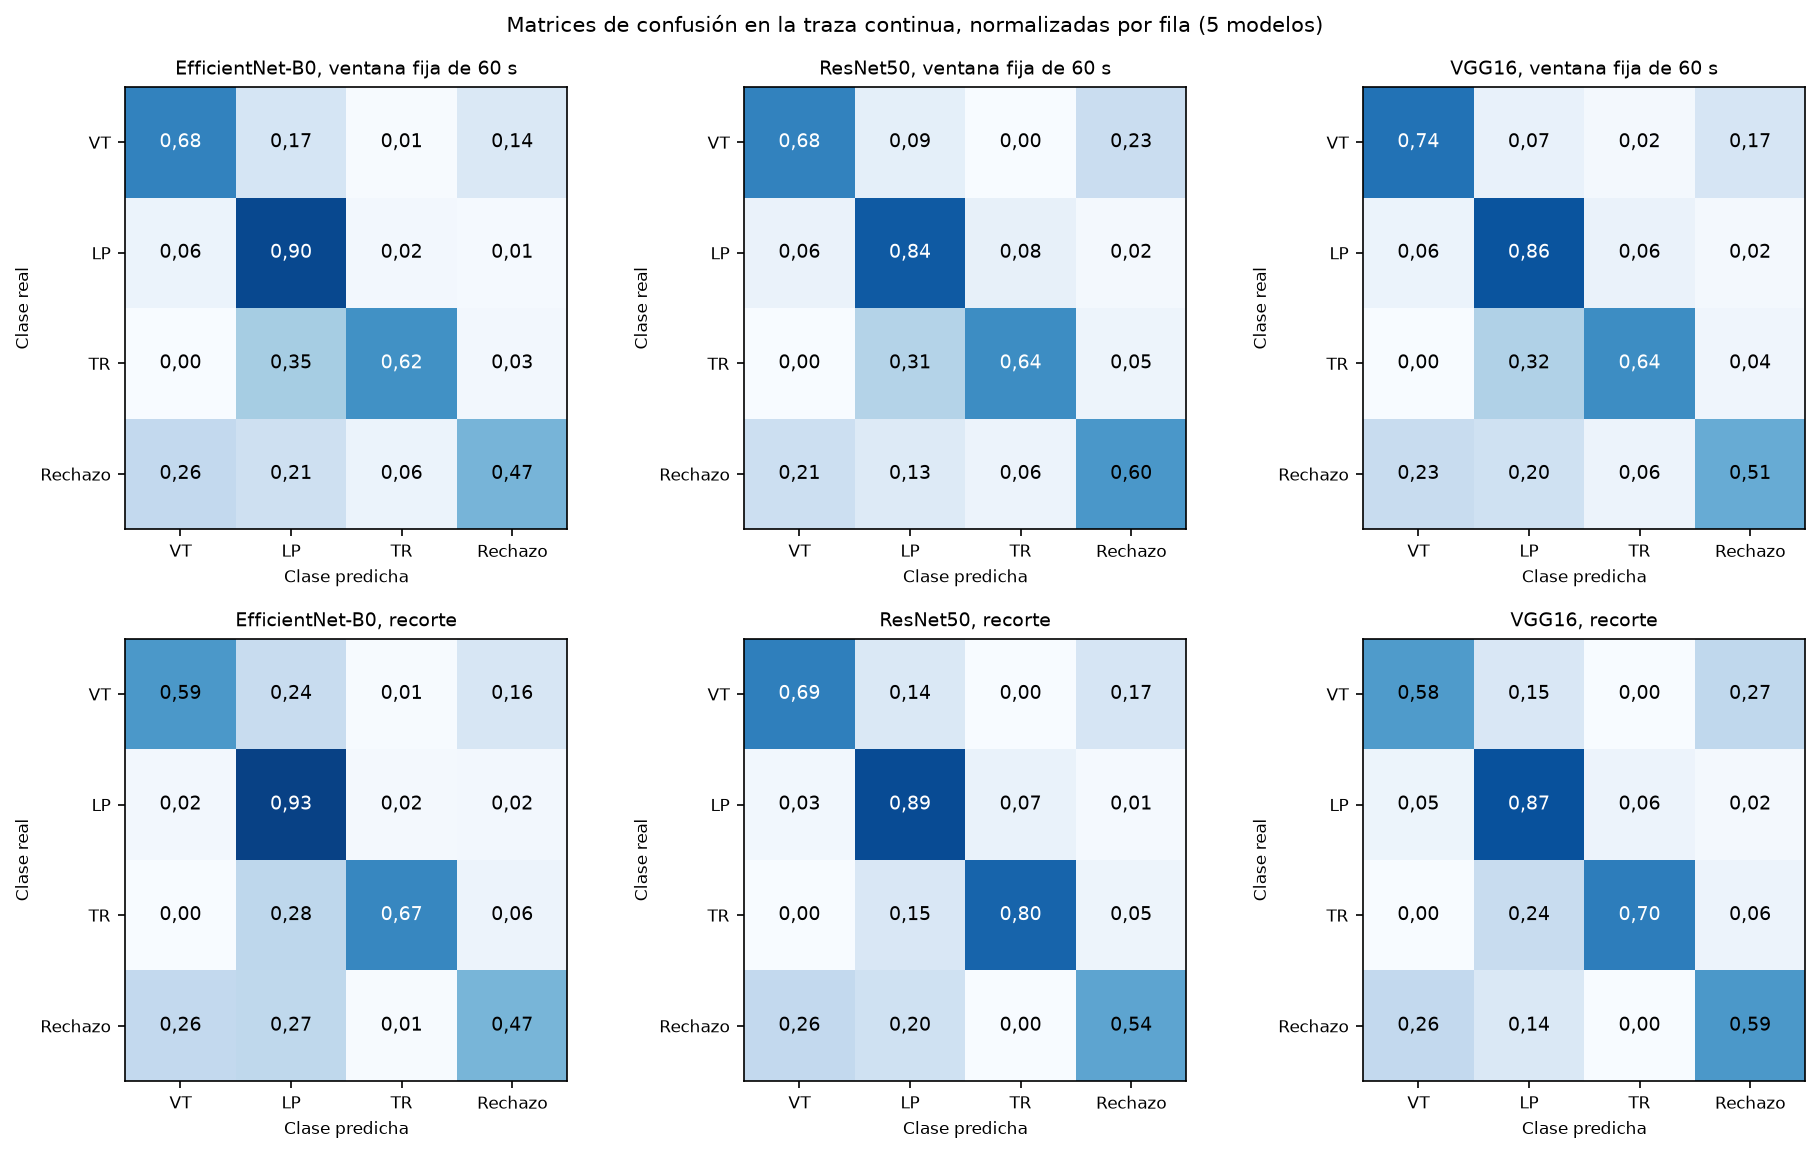
\includegraphics[width=\textwidth]{images/matrices_traza.png}
\caption{Matrices de confusión en la traza continua, normalizadas por fila
(suma de los cinco modelos de cada red). Arriba, con la ventana fija de
60\,s; abajo, con el recorte.}
\label{fig:res-matrices-traza}
\end{figure}

Los 855 recortes sin caja son 87,8 por hora de registro. El clasificador manda
a la clase de rechazo solo una parte de ellos: los que llama volcánicos son
entre 60,0 y 67,9 por hora con el recorte, según la red. Entre los cinco
modelos de una misma red esta cifra varía mucho; en ResNet50 va de 31,3 a 74,6
por hora.

\subsection{Tiempo de procesamiento}
\label{subsec:res-tiempo}

El Cuadro~\ref{tab:res-tiempo} da el tiempo de cada etapa sobre las 9,74 horas
de la traza, medido en el procesador del computador de trabajo, sin tarjeta
gráfica. La clasificación se da por modelo; en la evaluación se corrieron los
cinco modelos de cada red.

\needspace{9\baselineskip}
{\small
\begin{longtable}{lrr}
\caption{Tiempo de cada etapa sobre las 9,74 horas de la traza continua
(1.155 recortes).}\label{tab:res-tiempo}\\
\cabecera{\textbf{Etapa} & \textbf{Tiempo total (s)} & \textbf{Por recorte (ms)}}{3}
Detección con PhaseNet & 10,3 & --- \\
Recorte por energía & 0,3 & --- \\
Espectrogramas e imágenes & 13,1 & 11 \\
Clasificación con EfficientNet-B0 & 23,5 & 20,4 \\
Clasificación con ResNet50 & 52,1 & 45,1 \\
Clasificación con VGG16 & 78,1 & 67,6 \\
\end{longtable}
}

Con un modelo de EfficientNet-B0, la cadena completa procesa las 9,74 horas
en 47,2\,s, unas 740 veces más rápido que el tiempo real. Con ResNet50 toma
75,8\,s (unas 460 veces) y con VGG16, 101,8\,s (unas 340 veces). La red es la
etapa más lenta en las tres, y EfficientNet-B0, la red liviana, clasifica más
de tres veces más rápido que VGG16.

% =====================================================================
\section{Comprobaciones de la diferencia entre test y la traza}
\label{sec:res-comprobaciones}

El clasificador acierta menos en la traza continua que en test. Para acotar
por qué, se hicieron cuatro comprobaciones.

La primera es que la traza no se haya usado para entrenar. Ninguna de las
6.285 ventanas etiquetadas de origen, de las que salen las 5.669 con las tres
componentes completas, comparte tiempo con los tres tramos de la traza. La
traza no participó en el entrenamiento ni en la elección de la configuración
del clasificador.

La segunda es si la diferencia puede deberse al azar, porque en la traza hay
pocos recortes por clase. El Cuadro~\ref{tab:res-wilson} da, para cada red, la
sensibilidad de clasificación en la traza con su intervalo de confianza del
95\,\% (el promedio de los intervalos de los cinco modelos) y, al lado, el
promedio de test.

\needspace{9\baselineskip}
{\small
\setlength{\tabcolsep}{3pt}
\begin{longtable}{llrrlrl}
\caption{Sensibilidad de clasificación con el recorte en la traza, con su
intervalo de confianza del 95\,\%, y en test.}\label{tab:res-wilson}\\
\cabecera{\textbf{Red} & \textbf{Clase} & \textbf{Recortes} & \textbf{Traza} & \textbf{Intervalo} & \textbf{Test} & \textbf{¿Test dentro?}}{7}
EfficientNet-B0 & VT & 35 & 0,594 & [0,431; 0,739] & 0,893 & No \\
 & LP & 50 & 0,932 & [0,830; 0,972] & 0,869 & Sí \\
 & TR & 24 & 0,667 & [0,469; 0,818] & 0,764 & Sí \\
 & Rechazo & 40 & 0,465 & [0,322; 0,614] & 0,853 & No \\
\midrule
ResNet50 & VT & 35 & 0,691 & [0,528; 0,817] & 0,910 & No \\
 & LP & 50 & 0,892 & [0,778; 0,950] & 0,812 & Sí \\
 & TR & 24 & 0,800 & [0,606; 0,911] & 0,831 & Sí \\
 & Rechazo & 40 & 0,540 & [0,395; 0,678] & 0,857 & No \\
\midrule
VGG16 & VT & 35 & 0,583 & [0,421; 0,728] & 0,889 & No \\
 & LP & 50 & 0,872 & [0,753; 0,938] & 0,834 & Sí \\
 & TR & 24 & 0,700 & [0,501; 0,844] & 0,811 & Sí \\
 & Rechazo & 40 & 0,595 & [0,443; 0,731] & 0,904 & No \\
\end{longtable}
}

En VT y en el rechazo, el valor de test queda fuera del intervalo de la traza
en las tres redes: esa caída no se explica por el tamaño de la muestra. En LP y
TR el valor de test queda dentro del intervalo, así que con estos datos no se
puede decir que esas clases rindan distinto. Con la ventana fija de 60\,s pasa
lo mismo.

La tercera es si los recortes de la traza están peor delimitados que los de
test. No lo están: la mediana del IoU de los recortes con etiqueta de clase es
0,64 en test y 0,63 en la traza, y la parte con IoU de 0,5 o más es 0,75 y
0,71.

La cuarta mira, dentro de test, cómo cambia la sensibilidad según la posición
y la calidad del recorte. Las ventanas etiquetadas traen, además de la caja
principal al centro, cajas extra descentradas. El
Cuadro~\ref{tab:res-principal} compara las dos, y el
Cuadro~\ref{tab:res-iou-test} separa por IoU del recorte.

\needspace{9\baselineskip}
{\small
\setlength{\tabcolsep}{4pt}
\begin{longtable}{llrrrr}
\caption{Test con el recorte: sensibilidad por clase (promedio de los cinco
modelos) según el tipo de caja.}\label{tab:res-principal}\\
\cabecera{\textbf{Red} & \textbf{Caja} & \textbf{VT} & \textbf{LP} & \textbf{TR} & \textbf{Rechazo}}{6}
EfficientNet-B0 & Principal & 0,899 & 0,885 & 0,852 & 0,869 \\
 & Extra & 0,856 & 0,857 & 0,498 & 0,737 \\
ResNet50 & Principal & 0,919 & 0,853 & 0,914 & 0,869 \\
 & Extra & 0,847 & 0,783 & 0,584 & 0,774 \\
VGG16 & Principal & 0,896 & 0,867 & 0,887 & 0,913 \\
 & Extra & 0,842 & 0,811 & 0,584 & 0,837 \\
\midrule
Recortes & Principal & 293 & 281 & 183 & 282 \\
 & Extra & 43 & 395 & 61 & 38 \\
\end{longtable}
}

\needspace{9\baselineskip}
{\small
\setlength{\tabcolsep}{4pt}
\begin{longtable}{llrrrr}
\caption{Test con el recorte: sensibilidad por clase (promedio de los cinco
modelos) según el IoU del recorte con su caja.}\label{tab:res-iou-test}\\
\cabecera{\textbf{Red} & \textbf{IoU} & \textbf{VT} & \textbf{LP} & \textbf{TR} & \textbf{Rechazo}}{6}
EfficientNet-B0 & 0,3 a 0,5 & 0,919 & 0,886 & 0,590 & 0,791 \\
 & 0,5 a 0,7 & 0,936 & 0,880 & 0,833 & 0,876 \\
 & 0,7 o más & 0,831 & 0,852 & 0,918 & 0,881 \\
ResNet50 & 0,3 a 0,5 & 0,947 & 0,830 & 0,709 & 0,804 \\
 & 0,5 a 0,7 & 0,944 & 0,819 & 0,890 & 0,879 \\
 & 0,7 o más & 0,848 & 0,799 & 0,930 & 0,879 \\
VGG16 & 0,3 a 0,5 & 0,933 & 0,830 & 0,664 & 0,857 \\
 & 0,5 a 0,7 & 0,920 & 0,849 & 0,887 & 0,920 \\
 & 0,7 o más & 0,829 & 0,823 & 0,928 & 0,926 \\
\midrule
Recortes & 0,3 a 0,5 & 72 & 126 & 97 & 91 \\
 & 0,5 a 0,7 & 140 & 250 & 67 & 140 \\
 & 0,7 o más & 124 & 300 & 80 & 89 \\
\end{longtable}
}

Las cajas extra se clasifican peor que las principales, sobre todo en TR
(entre 0,50 y 0,58 contra entre 0,85 y 0,91). Las cajas extra difieren
también en otras cosas, como ser eventos secundarios de su ventana, así que
esta comparación no aísla el efecto de que el evento esté descentrado. En la
traza, cada recorte se clasifica en una ventana centrada en él, como las cajas
principales. Por IoU, TR depende mucho del recorte: con IoU entre 0,3 y 0,5 se
acierta entre 0,59 y 0,71, y con 0,7 o más, entre 0,92 y 0,93. En LP la
sensibilidad casi no cambia con el IoU, y en VT baja algo con IoU de 0,7 o
más.

Quedan sin medir dos posibles causas de la caída en VT y en el rechazo: que el
catálogo de la traza y el de las ventanas etiquetadas asignen las clases con
criterios distintos, y que los tramos de la traza correspondan a épocas o
condiciones del volcán distintas de las del entrenamiento. Se discuten en el
Capítulo~\ref{cap:discusion}.
